\documentclass[11pt]{exam} 
\usepackage{answers, amsthm, amsmath, amssymb, mathrsfs} \pagestyle{head} \firstpageheader{Math 228}{\bf Practice Problems 2: Quantifiers and Set Theory \\ Hints and Answers}{Spring 2013} \Newassociation{answer}{Ans}{Practice02-Quantifiers_Sets-solutions} 
 \def\d{\displaystyle}
\def\?{\reflectbox{?}}
\def\b#1{\mathbf{#1}}
\def\f#1{\mathfrak #1}
\def\c#1{\mathcal #1}
\def\s#1{\mathscr #1}
\def\r#1{\mathrm{#1}}
\def\N{\mathbb N}
\def\Z{\mathbb Z}
\def\Q{\mathbb Q}
\def\R{\mathbb R}
\def\C{\mathbb C}
\def\F{\mathbb F}
\def\A{\mathbb A}
\def\X{\mathbb X}
\def\E{\mathbb E}
\def\O{\mathbb O}
\def\U{\mathcal U}
\def\pow{\mathcal P}
\def\inv{^{-1}}
\def\nrml{\triangleleft}
\def\st{:}
\def\~{\widetilde}
\def\rem{\mathcal R}
\def\sigalg{$\sigma$-algebra }
\def\Gal{\mbox{Gal}}
\def\iff{\leftrightarrow}
\def\Iff{\Leftrightarrow}
\def\land{\wedge}
\def\And{\bigwedge}
\def\AAnd{\d\bigwedge\mkern-18mu\bigwedge}
\def\Vee{\bigvee}
\def\VVee{\d\Vee\mkern-18mu\Vee}
\def\imp{\rightarrow}
\def\Imp{\Rightarrow}
\def\Fi{\Leftarrow}

%\def\={\equiv}
\def\var{\mbox{var}}
\def\mod{\mbox{Mod}}
\def\Th{\mbox{Th}}
\def\sat{\mbox{Sat}}
\def\con{\mbox{Con}}
\def\bmodels{=\joinrel\mathrel|}
\def\iffmodels{\bmodels\models}
\def\dbland{\bigwedge \!\!\bigwedge}
\def\dom{\mbox{dom}}
\def\rng{\mbox{range}}
\DeclareMathOperator{\wgt}{wgt}


\def\bar{\overline}


\newcommand{\vtx}[2]{node[fill,circle,inner sep=0pt, minimum size=4pt,label=#1:#2]{}}
\newcommand{\va}[1]{\vtx{above}{#1}}
\newcommand{\vb}[1]{\vtx{below}{#1}}
\newcommand{\vr}[1]{\vtx{right}{#1}}
\newcommand{\vl}[1]{\vtx{left}{#1}}
\renewcommand{\v}{\vtx{above}{}}

\def\circleA{(-.5,0) circle (1)}
\def\circleAlabel{(-1.5,.6) node[above]{$A$}}
\def\circleB{(.5,0) circle (1)}
\def\circleBlabel{(1.5,.6) node[above]{$B$}}
\def\circleC{(0,-1) circle (1)}
\def\circleClabel{(.5,-2) node[right]{$C$}}
\def\twosetbox{(-2,-1.4) rectangle (2,1.4)}
\def\threesetbox{(-2.5,-2.4) rectangle (2.5,1.4)}
\newcommand{\twoline}[2]{\begin{pmatrix}#1 \\ #2 \end{pmatrix}}

\usepackage{tikz, multicol}
\renewenvironment{Ans}[1]{\setcounter{question}{#1}\addtocounter{question}{-1}\question }{}
\begin{document}
 \begin{questions}
\begin{Ans}{1}
     \begin{parts}
	\part $\neg \exists x (E(x) \and O(x))$
	\part $\forall x (E(x) \imp O(x+1))$
	\part $\exists x(P(x) \and E(x))$ (where $P(x)$ means ``$x$ is prime'')
	\part $\forall x \forall y \exists z(x < z < y \vee y < z < x)$
	\part $\forall x \neg \exists y (x < y < x+1)$
    \end{parts}
  
\end{Ans}
\begin{Ans}{2}
    \begin{parts}
	\part Any even number plus 2 is an even number.
	\part For any $x$ there is a $y$ such that $\sin(x) = y$.  In other words, every number $x$ is in the domain of sine.
	\part For every $y$ there is an $x$ such that $\sin(x) = y$.  In other words, every number $y$ is in the range of sine (which is false).
	\part For any numbers, if the cubes of two numbers are equal, then the numbers are equal.
      \end{parts}
  
\end{Ans}
\begin{Ans}{3}
    \begin{parts}
	\part $\forall x \exists y (O(x) \and \neg E(y))$
	\part $\exists x \forall y (x \ge y \vee \forall z (x \ge z \and y \ge z))$
	\part There is a number $n$ for which every other number is strictly greater than $n$.
	\part There is a number $n$ which is not between any other two numbers.
      \end{parts}
  
\end{Ans}
\begin{Ans}{4}
    \begin{parts}
	\part $A \cap B = \{3,4,5\}$.  %Find $A \cap B$.
	\part $A \cup B = \{1,2,3,4,5,6,7\}$. %Find $A \cup B$.
	\part $A \setminus B = \{1,2\}$. %Find $A \setminus B$.
	\part Yes.  %Is $C \subseteq A$?
	\part No. %Is $C \subseteq B$?
    \end{parts}
  
\end{Ans}
\begin{Ans}{5}
    \begin{parts}
  %Find $A \cap B$
	\part $A \cap B = \{4,6,8,10,12\}$
  % Find $A \cup B$.
	\part $A \cup B = \{x \in \N \st (3 \le x \le 13) \vee x \mbox{ is even}\}.$ (the set of all natural numbers which are either even or between 3 and 13 inclusive).
  %Find $B \cap C$.
	\part $B \cap C = \emptyset$.
  %Find $B \cup C$.
	\part $B \cup C = \N$.
      \end{parts}
  
\end{Ans}
\begin{Ans}{6}
    For example, $A = \{2,3,5,7,8\}$ and $B = \{3,5\}$.
  
\end{Ans}
\begin{Ans}{7}
    Let $A = \{1,2,3\}$ and $B = \{1,2,3,4,5,\{1,2,3\}\}$
  
\end{Ans}
\begin{Ans}{8}
    \begin{parts}
	\part No.
	\part No.
	\part $2\Z \cap 3\Z$ is the set of all integers which are multiples of both 2 and 3 (so multiples of 6).  Therefore $2\Z \cap 3\Z = \{x \in \Z \st \exists y\in \Z(x = 6y)\}$.
	\part $2\Z \cup 3\Z$.
 \end{parts}
  
\end{Ans}
\begin{Ans}{9}
    The set of primes.
  
\end{Ans}
\begin{Ans}{10}
      \begin{parts}
	  \def\circleA{(-.5,0) circle (1)}
	  \def\circleAlabel{(-1.5,.6) node[above]{$A$}}
	  \def\circleB{(.5,0) circle (1)}
	  \def\circleBlabel{(1.5,.6) node[above]{$B$}}
	  \def\circleC{(0,-1) circle (1)}
	  \def\circleClabel{(.5,-2) node[right]{$C$}}
	  \def\twosetbox{(-2,-1.5) rectangle (2,1.5)}
	  \def\threesetbox{(-2,-2.5) rectangle (2,1.5)}

	  \begin{multicols}{3}
	    \part  $A \cup \bar B$:

	    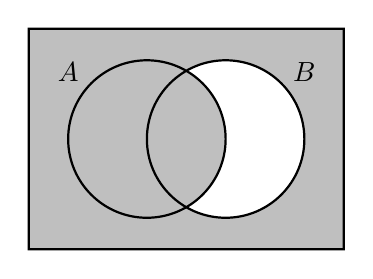
\begin{tikzpicture}[fill=gray!50]
	  %Fill A:
	  \fill \circleA;
	  %Fill \bar B:
	    \begin{scope}
	    \clip \circleB \twosetbox; %This defines the scope to everything in the twosetbox which is not in circleB.
	    \fill \twosetbox;
	    \end{scope}
	    \draw[thick] \circleA \circleAlabel \circleB \circleBlabel \twosetbox;
	  \end{tikzpicture}

	  \vfill

	  %
	  \part $\bar{(A \cup B)}$:

	  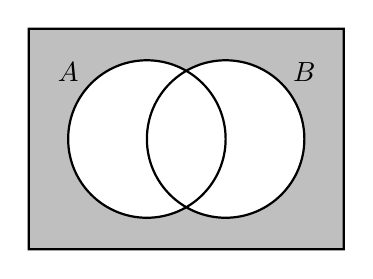
\begin{tikzpicture}[fill=gray!50]
	    \fill \twosetbox;
	    \fill[white] \circleA \circleB;
	    \draw[thick] \circleA \circleAlabel \circleB \circleBlabel \twosetbox;
	  \end{tikzpicture}

	  \columnbreak

	  %
	  \part $A \cap (B \cup C)$:

	  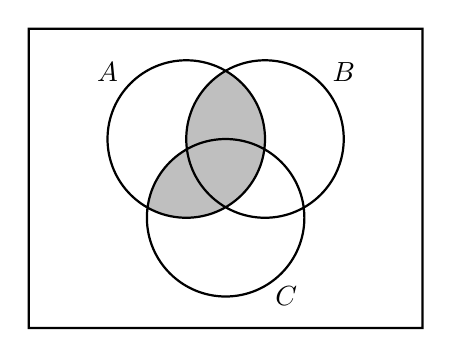
\begin{tikzpicture}[fill=gray!50]
	  \begin{scope}
	    \clip \circleA;
	    \fill \circleB \circleC;
	  \end{scope}
	  \draw[thick] \circleA \circleAlabel \circleB \circleBlabel \circleC \circleClabel \threesetbox;
	  \end{tikzpicture}

	  %
	  \part $(A \cap B) \cup C$:

	  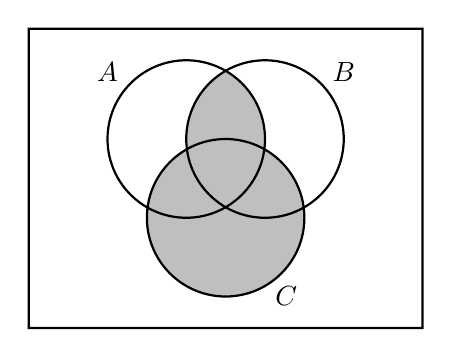
\begin{tikzpicture}[fill=gray!50]
	  \begin{scope}
	    \clip \circleA;
	    \fill \circleB;
	  \end{scope}
	  \fill \circleC;
	  \draw[thick] \circleA \circleAlabel \circleB \circleBlabel \circleC \circleClabel \threesetbox;
	  \end{tikzpicture}
	  \vfill
	  \columnbreak

	  %
	  \part $\bar A \cap B \cap \bar C$:

	  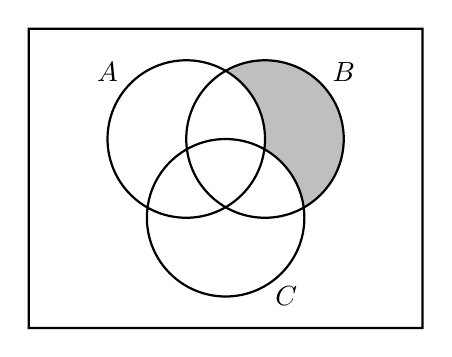
\begin{tikzpicture}[fill=gray!50]
	  \fill \circleB;
	  \begin{scope}
	    \clip \circleB;
	    \fill[white] \circleA \circleC;
	  \end{scope}

	  \draw[thick] \circleA \circleAlabel \circleB \circleBlabel \circleC \circleClabel \threesetbox;
	  \end{tikzpicture}

	  %
	  \part $(A \cup B) \setminus C$:

	  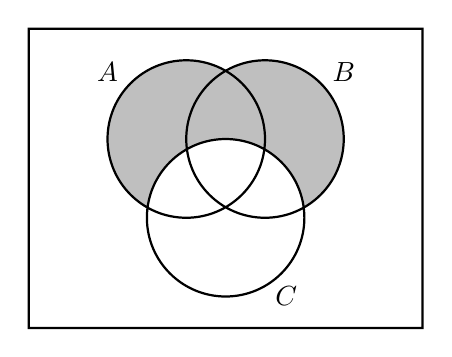
\begin{tikzpicture}[fill=gray!50]
	  \fill \circleA;
	  \fill \circleB;
	  \fill[white] \circleC;
	  \draw[thick] \circleA \circleAlabel \circleB \circleBlabel \circleC \circleClabel \threesetbox;
	  \end{tikzpicture}
	  \end{multicols}
	  \end{parts}
  
\end{Ans}
\begin{Ans}{11}
    For example, $A \cup B \cap \bar{(A \cap B)}$.  Note that $\bar{A \cap B}$ would almost work, but also contain the area outside of both circles.
  
\end{Ans}
\begin{Ans}{12}
      \begin{parts}
	  \part 34.
	  \part 103.
	  \part 8.
      \end{parts}
  
\end{Ans}
\begin{Ans}{13}
    $\pow(A) = \{\emptyset, \{a\}, \{b\}, \{c\}, \{a,b\}, \{a,c\}, \{b,c\}, \{a,b,c\}\}$.
  
\end{Ans}
\begin{Ans}{14}
      There are 10 singletons.  There are 45 doubletons (because $45 = 9+8+7+\cdots+2+1$).
  
\end{Ans}
\begin{Ans}{15}
      $\{2,3,5\}, \{1,2,3,5\}, \{2,3,4,5\}, \{2,3,5,6\}, \{1,2,3,4,5\}, \{1,2,3,5,6\}, \{2,3,4,5,6\}$, and $\{1,2,3,4,5,6\}$.
  
\end{Ans}
\begin{Ans}{16}
   For example $A = \{1,2,3,4\}$ and $B = \{5,6,7,8,9\}$.
  
\end{Ans}
\begin{Ans}{17}
    For example, $A = \{1,2,3\}$ and $B = \{2,3,4,5\}$.
  
\end{Ans}
\begin{Ans}{18}
      If $R$ is the set of red cards and $F$ is the set of face cards, we want to find $|R \cup F|$.  This is not simply $|R| + |F|$ because there are 6 cards which are both red and a face card; $|R \cap F| = 6$.  We find $|R \cup F| = 32$.
  
\end{Ans}
 \end{questions} \par \end{document}
